\documentclass[12pt, letterpaper]{article}
\usepackage{iarc_latex_style}
\usepackage{amssymb,amsmath,listings,url,verbatim,graphicx}

\title{Beohawk: Autonomous Quadrotor}
\begin{document}
\maketitle
\begin{people}
\name{Debjit Ghosh, Rustom Jehangir, Christopher Li, Keith McKay, Yujia Zhai}
\org{University of Southern California}

\end{people}

%1) Abstract	5
\begin{abstract}
In this paper, we introduce a Micro UAV system that can explore an unknown indoor space without the assistance of a positioning system such as GPS. The robot receives sensor measurements from cameras, sonar, and an infrared depth sensor.  Using SLAM, it handles the data probabilistically and generates a map of the environment, which is used for setting waypoints and avoiding obstacles.  The mechanical construction of the vehicle, low-level control, and sensor communication are also discussed in the paper.
\end{abstract}

%2) Introduction	5
%  a) Statement of the problem 
%  b) Conceptual solution to solve the problem
%    b1) Figure of overall system architecture 
%  c) Yearly Milestones
\section{Introduction}

%\subsection{Problem Statement}

For the $6^\text{th}$ International Aerial Robotics Competition, an autonomous aerial vehicle under 1.5 kilograms must explore an unknown office floor, localize itself according to the environment, identify and pick up a black USB drive, and return to a handler within the given time limit. The robot may also be intelligent enough to identify mission-related features, such as signs above rooms, or observe and avoid obstacles such as surveillance devices while traversing the hallways.

\subsection{Conceptual Solution}

The Aerial Robotics Team (ART) of the USC Robotics Society (USCRS) purposes a quadrotor design of its aerial robot vehicle, \textit{Beohawk}, which consists of four motors located symmetrically at each end of an X-shape frame (figure \ref{fig:beohawk}). The frame of the quadrotor was custom built by our team members to be within the required weight and size range. Various sensors, the on-board computer, and other facilities are located at the center of the frame. An off-board computing station is dedicated to the majority of computational tasks; it receives data from the on-board computer, processes the data to determine future movements of the robot, and publishes operating commands back. The communication is done over a standard 802.11n network. Both computers run mission-specific programs written by our team. These programs run on the Robotic Operating System (ROS) and take advantage of many packages and tools made available by public contributors. Utilizing inertial and visual data from various sensors and processing the data with state-of-the-art algorithms, we hope to perform stabilization, navigation and mission planning on the quadrotor to complete the challenge.

\begin{figure}[h]
\centering
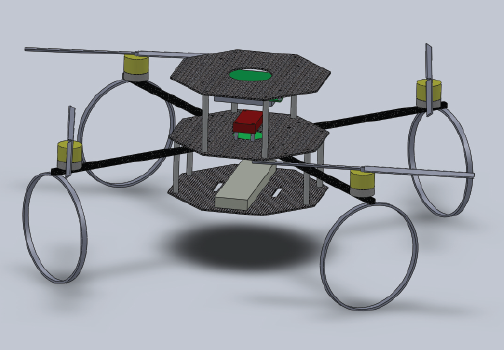
\includegraphics[width=10cm]{images/Beohawk_V3.png}
\captionit{SolidWorks render of Beohawk's main frame.  Four propellers provide lift.  Sensors and computers are located in the center of the quadrotor.} 
\label{fig:beohawk}
\end{figure}

\subsubsection{Figure of Overall System Architecture}

Figure \eqref{fig:architecture} shows the basic system architecture of the quadrotor. The quadrotor's low level control including stability, attitude control, altitude control, and position control are all performed by the low-level control board. This board is Arduino based and has sensor inputs and motor outputs. It also receives radio-control signals that allow control to be over-ridden by a human pilot.

\begin{figure}[h]
\centering
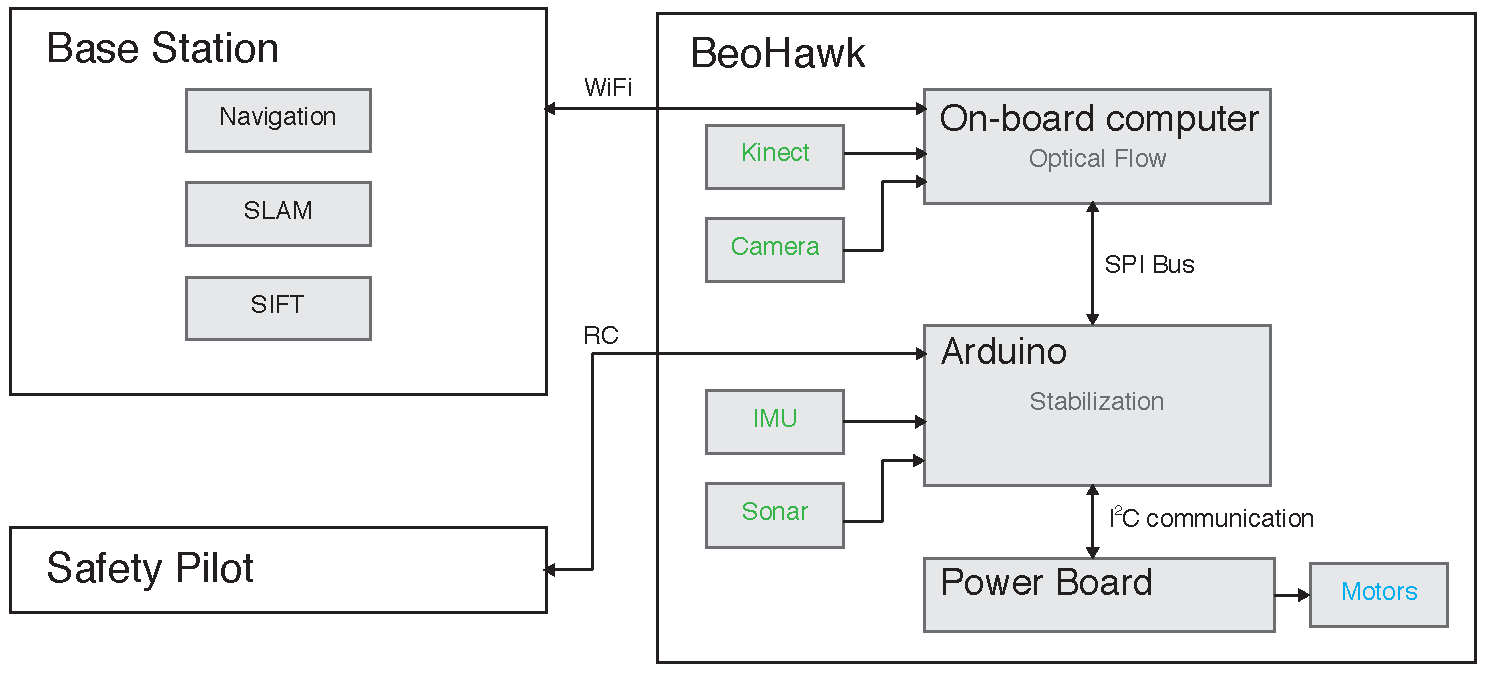
\includegraphics[width=14cm]{images/beohawk-system-arch.pdf}
\captionit{General architecture of the Beohawk control system.} 
\label{fig:architecture}
\end{figure}

\subsection{Yearly Milestones}

This is the USC Robotics Society's first appearance at IARC as well our first competition. Our hardware team has developed three models for the frame in the past two years. Our latest model uses strong, lightweight carbon fiber in the frame. The software team has researched algorithms for UAV stabilization and navigation, and has tried to develop 3D visual navigation systems through both a probabilistic approach and a graph approach, which will be discussed later in detail. Our electrical team has designed a customized circuit board to replace the commercialized alternatives (such as Arduino board). Regardless of the outcome of competition, we will continue refining hardware frames, circuit designs, software algorithms, and visualization interfaces.

% picuture of the frame (solidworks) 

%3) Air Vehicle	15
%  a) Propulsion and Lift System 
%  b) Guidance, Nav., and Control 
%    b1) Stability Augmentation System 
%    b2) Simultaneous Localization and Mapping
%    b3) Navigation
%    b4) Figure of control system architecture 
%    b5) Target Identification and Threat Avoidance
%  d) Flight Termination System
\section{Air Vehicle}

\subsection{Propulsion and Lift System}
\emph{Beohawk} has four rotors, each an equal distance from the quadrotor's center.  Two opposite motors spin clockwise and the other two spin counter-clockwise, which generates a net torque of zero.  Therefore, by increasing the speed of a pair of rotors spinning in one direction and decreasing the others, a yaw motion can be produced. Quadrotors are ideal for unmanned aerial vehicles because they have simple mechanics and require small rotors, which reduces the cost of the vehicle and power required to operate \cite{bib:quadrotor}.

\subsection{Guidance, Navigation, and Control}
\subsubsection{Stability Augmentation System}

The quadrotor vehicle is a statically unstable system that must be controlled by a stability control system. The attitude and rate of change of the vehicle are measured by accelerometers and gyroscopes. Additionally, the vehicle's altitude and drift from original position are measured using a sonar and an optical flow sensor. With this combination of sensors, the vehicle is able to hold a set location without significant drift.

Several sensor measurements have been proven to have strong, reliable relationships with the position (translation and/or rotation) of the robot. Monitoring their changes can give us very useful knowledge about how much the robot drifts from its original position. We use the direct-cosine matrix algorithm (DCM) to provide an optimized result of the real-time orientation of the robot. This algorithm utilizes the three-axis linear acceleration and angular velocity measurements from the onboard inertial measurement unit (IMU). Since linear acceleration readings from the accelerometer are more accurate in the long term while angular velocity readings from the gyroscope tend to drift through time, the DCM algorithm uses acceleration information to correct the gyroscope readings, thereby giving almost drift-free information about the robot's orientation. In addition, we also use a downward-facing camera to calculate the optical flow of salient, time-independent visual features. By doing so, we are able to figure out the motion trajectory of this camera, a technique called ``structure from motion''. A sonar sensor is also mounted on the bottom of the quadrotor. It measures a much more accurate altitude reading, and is used to improve the results of the optical flow algorithm. The combination of the DCM algorithm for the IMU and the structure-from-motion technique for the visual camera allows us to keep track of robot's linear and angular position in real time.

\begin{figure}[h]
\centering
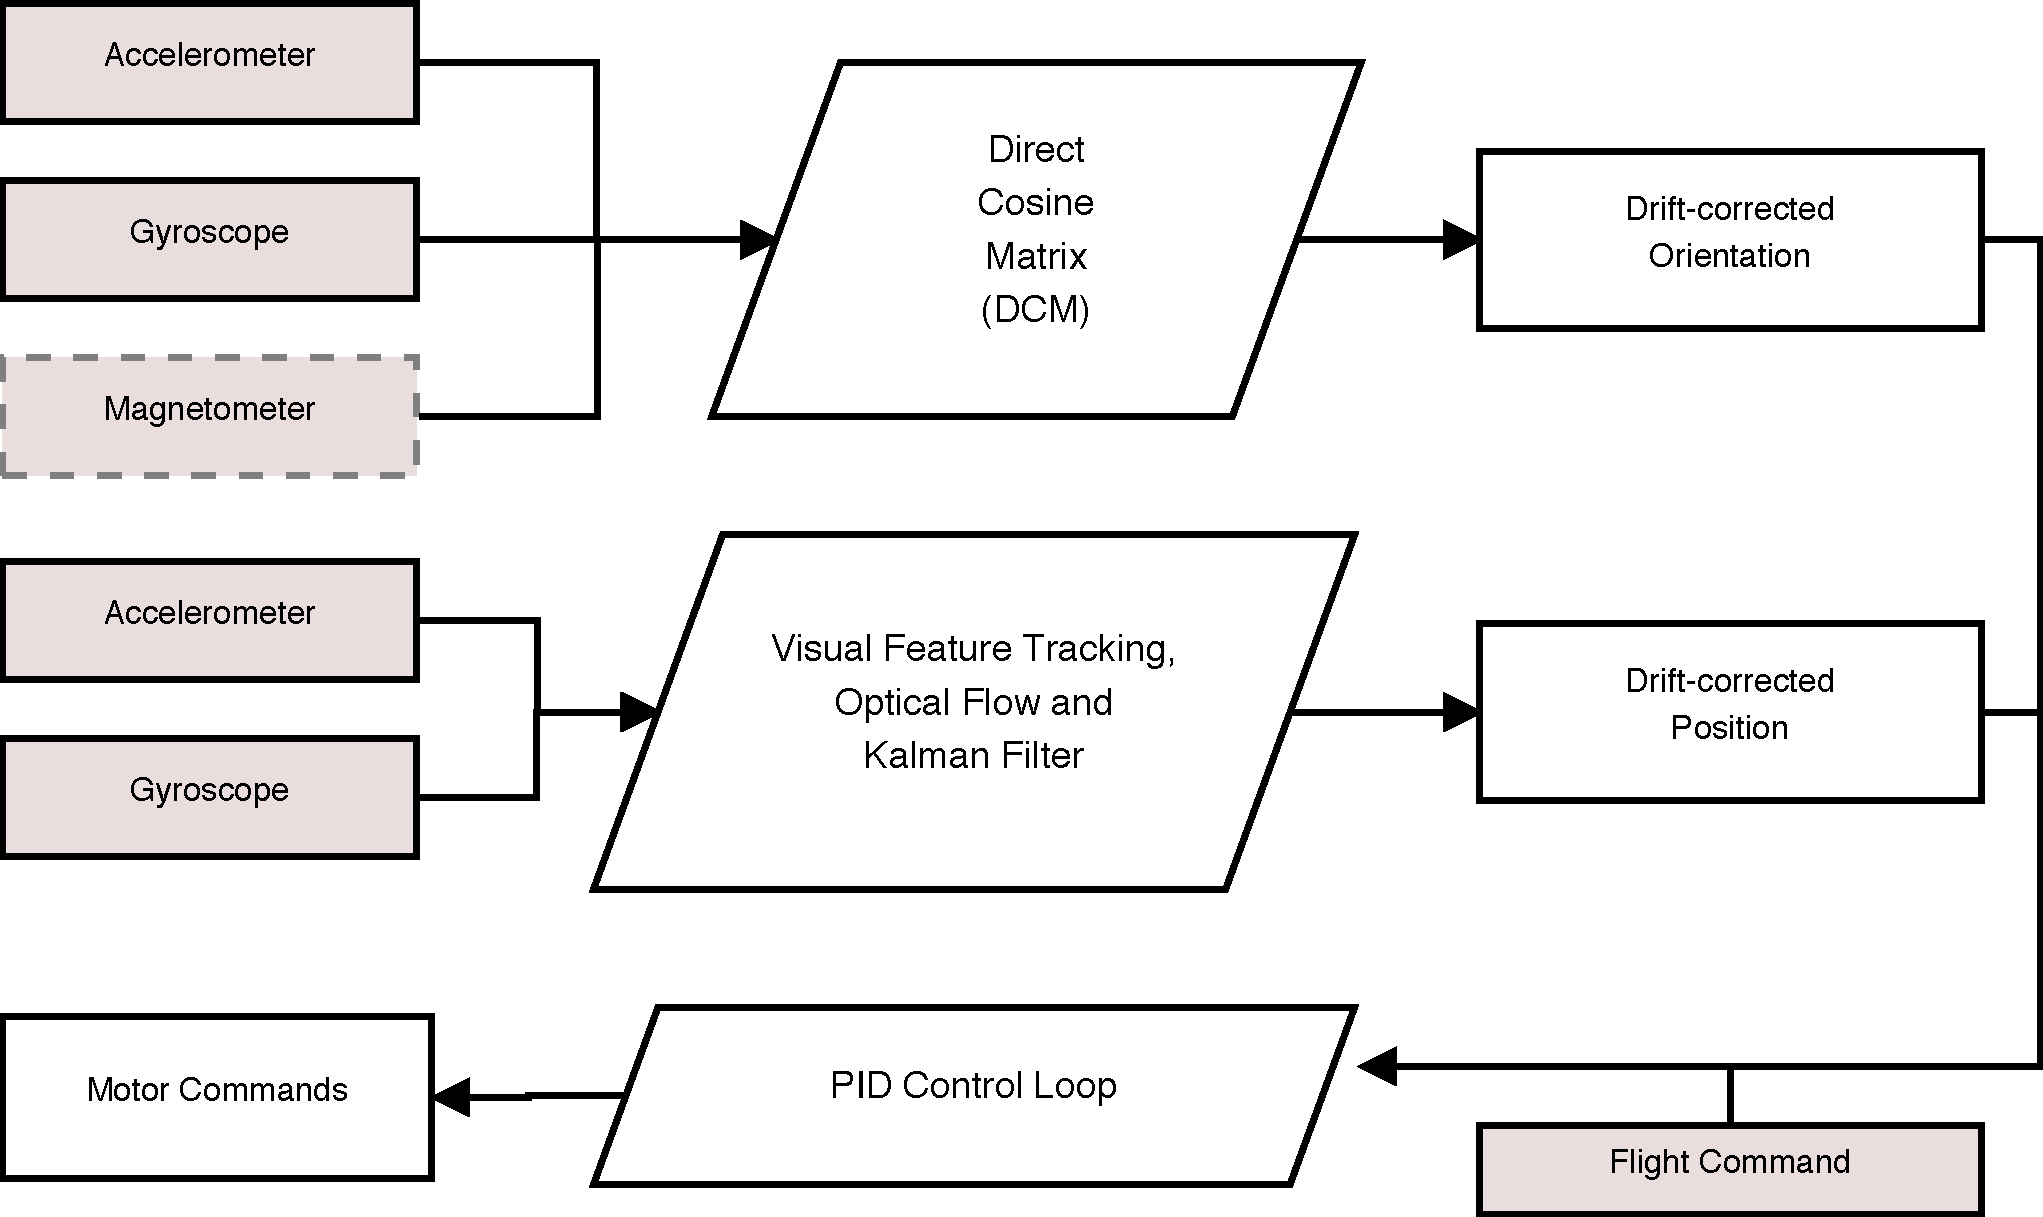
\includegraphics[width=12cm]{images/PID.pdf}
\captionit{Feedback of drift information into the PID loop.} 
\label{fig:PID}
\end{figure}

Finally, this system uses a PID control loop to handle the stabilization issue given these position-related measurements (figure \ref{fig:PID}). This control loop constantly updates the motor speeds based on the difference between perceived and desired attitude and position. The system also uses an Extended Kalman Filter to correct the position estimation from optical flow algorithm in order to get rid of unpredicted noises in visual feature recognition and matching. The positional error generated by the optical flow algorithm is used in another PID control system to control the position of the vehicle. In fact, all vehicle movements are perceived as errors in position instead of as goals. The control system then applies the appropriate motor commands to correct the positional error and move to the next location.

\subsubsection{Simultaneous Localization and Mapping}

Simultaneous localization and mapping (SLAM) has been the central problem for autonomous robots in unknown environments. The purpose of the SLAM is to predict, as accurately as possible, the position of the robot based on its knowledge of the surrounding environment.  To do this, we must obtain the 3D position of visual salient features and calculate the affine transformation of the camera through time. Combining this with the gyroscope and optical flow readings, we can set up an optimization system to reduce the effect of random errors.

\begin{figure}[h]
\centering
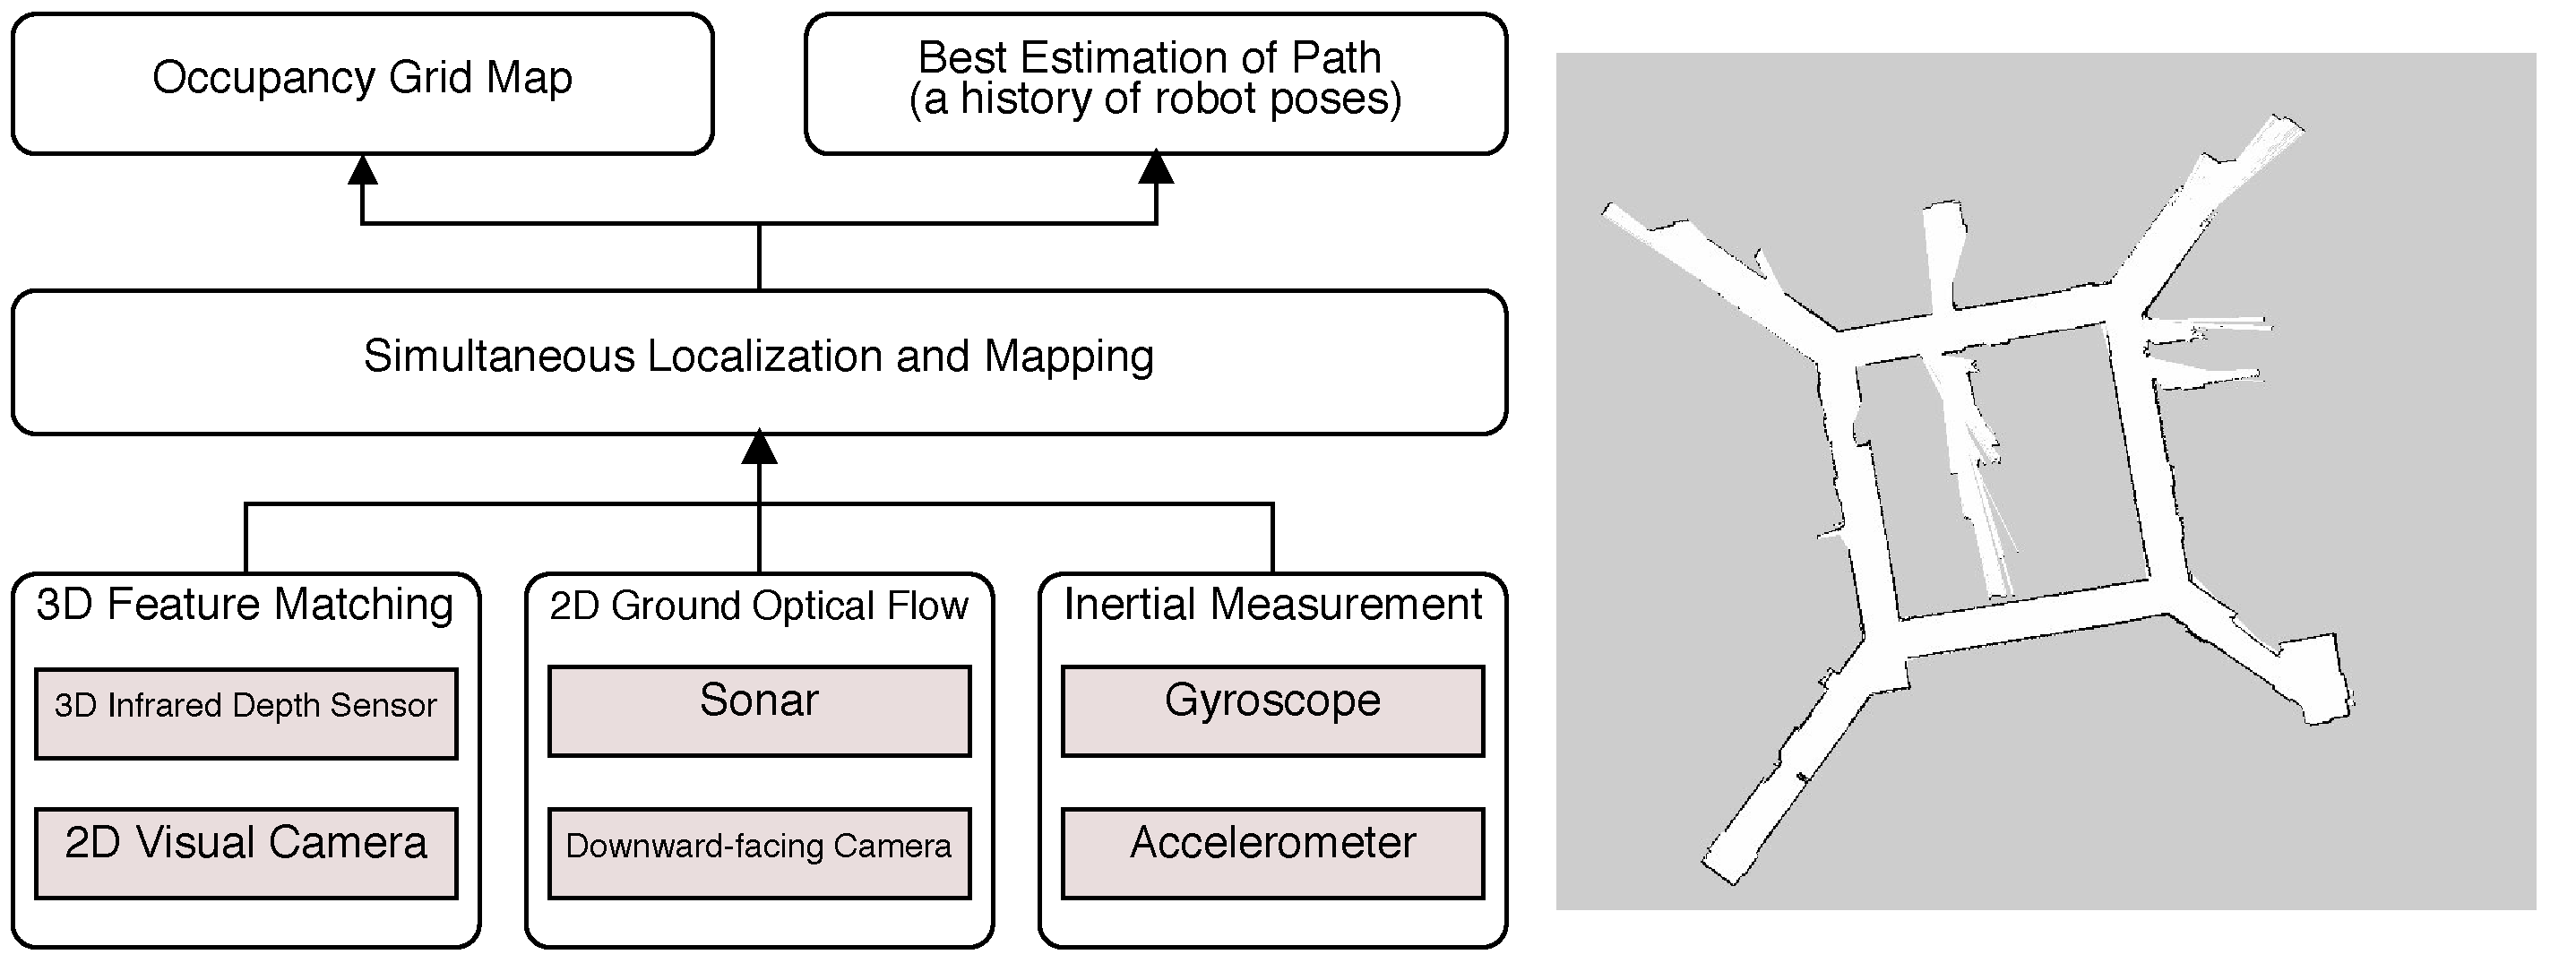
\includegraphics[width=16cm]{images/SLAM.pdf}
\captionit{Left: The inputs and outputs of SLAM. Right: Our robotics lab as seen through the SLAM algorithm.} 
\label{fig:slam}
\end{figure}

In this project, we use an infrared-powered depth camera that can tell how far one given point is away from the camera. Combining this depth camera with a traditional RGB camera, we are able to create a 3D model (or ``point cloud'') of the visual perception as well as matching them in 3D to figure out the camera trajectory (figure \ref{fig:slam}). Because matching every point across point clouds requires a great amount of time and energy to process, we only match the points representing the same object in the real world from different clouds. Singular value decomposition is used to process the matching result and to produce the translation and rotation matrix.

Results from the 3D visual matching and transformation calculation described above are the major source of pose estimation. To further optimize the localization result, we will use either a probabilistic system or a graph system. The probabilistic system utilizes a Monte-Carlo theory based particle filter to generate most possible result; it only depends on the probability distribution of pose at the most recent time. The graph system, on the other hand, creates a graph where vertices are the poses and edges are the transformation constraints between poses. The graph system doesn't require us to simulate the probability model of system, control, or sensing inputs, but requires more computational power to manage the graph.

\subsubsection{Navigation}

While we can get the 6 degree-of-freedom position and orientation status of the robot, we only need the Navigation done in 2D, because the place our robot will explore is a single plane floor. For this, we use the official 2D navigation package from ROS.

The ROS navigation stack takes sensor data, the SLAM map, a TF transformation tree, and visual odometry information as inputs.  Internally, it maintains costmaps and planners used to calculate the least expensive route.  

Operating alongside the navigation stack is the mission planner, which runs as a ROS node on the base station.  The mission planner is a state machine that keeps track of current goals.  It broadcasts a topic that contains the current mission (e.g. explore a hallway, find the security office, pick up the flash drive) as well as a goal for the navigation stack.

\subsubsection{Figure of Control System Architecture}

\begin{figure}[h]
\centering
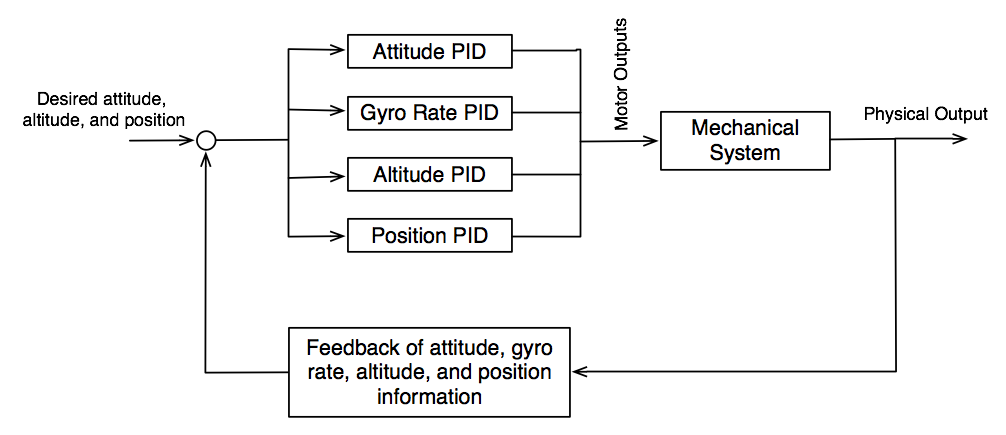
\includegraphics[width=14cm]{images/Control-System-Diagram.png}
\captionit{Control system architecture. } 
\label{fig:controlsystem}
\end{figure}

Figure \ref{fig:controlsystem} shows a general diagram of the control system architecture for vehicle control and stability. The feedback control system uses measured attitude, gyro rate, altitude, and position information to correct the vehicle's position and orientation to the desired position and orientation. The PID control system relies on hand-tuned constants that were found through trial and error during a variety of tests. 

PID control systems were used for all control movements because of their simplicity and effectiveness. All commands sent from the navigation computer are interpreted as errors relative to the current state of the vehicle. The PID control system is a simple way to reduce such errors and can therefore be used to control all aspects of vehicle movement.

\subsubsection{Target Identification and Threat Avoidance}

Since the USB is a black object located on a white table surface, an edge or contrast detection algorithm will easily identify the USB as a salient feature. While the 3D visual sensor may not be enough accurate to tell the dimension of the USB, it can sense the much larger box containing the USB and therefore helps in target identification. 

Identifying the signatures on the doors to different rooms is a tough task, because arabic characters are difficult to identify with traditional OCR technology, especially since the quadrotor may look at the signature from unknown perspective, which results in an affine transformation of the signature image that. \textit{Beohawk} uses a scale/rotation invariant feature detection algorithm called ``SIFT'' to tackle this problem. The algorithm tries to match the picture it sees and the template in the database by trying numerous cases of different transformations. This algorithm has been proven successful in matching pictures regardless of scale, rotation or gradient constraints \cite{bib:sift}.

\subsection{Flight Termination System}
Because the RC controller communicates directly with the Arduino, the safety pilot can terminate the operation of the quadrotor in the event it is needed. One channel of the RC transmitter is connected to a switch that transfers control from the computer system to the human pilot.

%4) Payload	15
%  a) Sensor Suite 
%  c) Power Management System 
%  b) Communications 

\section{Payload}
\subsection{Sensor Suite}

\subsubsection{Inertial Measurement Unit}

The sensor board is based on the commercially available ``Ardupilot Mega" which provides an Inertial Measurement Unit or IMU. The sensors are analog MEMS-based sensors that provide high sensitivity, high bandwidth measurements used to calculate attitude of the vehicle. This sensor board was used because of its commercial availability and extensive community support and software.

\subsubsection{2D Visual Camera}

Using a downward facing camera, the quadrotor runs an optical flow algorithm on the x86 processor to reduce drift.  A second, front-facing camera captures pictures for reading the signs above the doors.  The images are published through the wireless network to the base station, which runs SIFT to detect the Chief of Security's office via the sign above the door. The front camera is also responsible for detecting the blue security light.  The bottom camera is used to identify the flash drive.

\subsubsection{3D Infrared Depth Camera}

\begin{figure}[h]
\centering
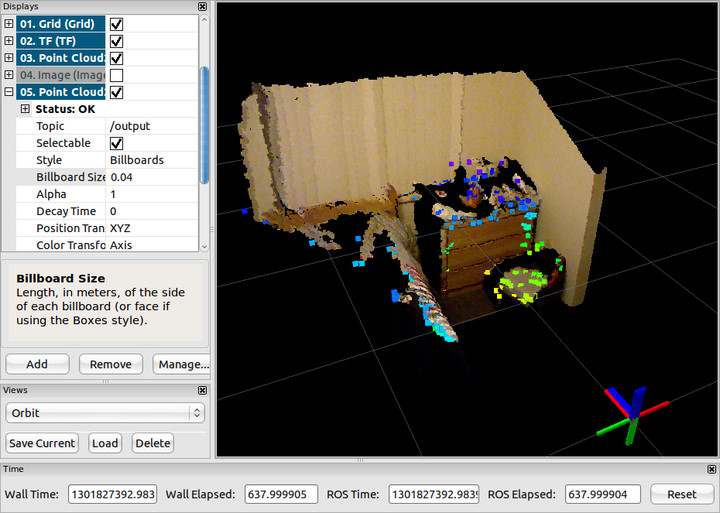
\includegraphics[width=14cm]{images/point-cloud.jpg}
\captionit{Depth information superimposed on 2D camera data. The color of each point indicates relative depth, with red being closest and violet being farthest.} 
\label{fig:point-cloud}
\end{figure}

We have installed a Microsoft Kinect on the quadrotor as a novel solution to the SLAM and navigation problem. This device serves as a depth sensing camera, which provides an image of 640x480 points at 15Hz; each point contains information at 2048 levels of sensitivity. The camera is mounted downward at a 45$^\circ$ angle from the horizon.

\subsubsection{Sonar}

Though the quadrotor has an estimate of altitude from infrared depth camera, the quadrotor also employs a downward-facing sonar to determine its altitude.

\subsection{Communications}

An IEEE 802.11n network is established between an on-board computer and a ground station. This network is time-synchronized and supports functionalities on both machines to communicate with each other through the ROS message system. While camera sensors are well supported by ROS, inertial sensor data and motor command have to go through serial communication. Since serial communication has not been implemented in ROS distribution so far, we developed a serial communication node that provides a protocol for exchanging messages safely through serial communication, which greatly improves the reliability of whole system. We use a RS 232 based connection between the on-board computer and ArduPilot to communicate the motor commands as well as receive position/orientation information from the various on-board sensors. The sensor board passes rotor commands to the power board with I$^2$C technology. It also connects to an RC control device that can be used for manual override. Visual sensing streams are read at 30 Hz for 2D images and 15 Hz for 3D depth images over USB.

\subsection{Power Management System}

Beohawk is powered by a 7.4V 5000mAh Lithium-Polymer battery pack, which provides enough energy to run at least ten minutes. A power regulator board controls the battery and motor speed. The power board uses a processor and I2C communication to send commands to the motors. The motors and then connected through PWM ports. In the event of low power, the base station initiates a controlled descent to avoid damage to the quadrotor.

%5) Operations	10
%  a) Flight Preparations 
%    a1) Checklist(s) 
%  b) Man/Machine Interface
\section{Operations}

\subsection{Flight Preparations}
Before any flight is performed, batteries must be charged an an able human operator must be available to assume the control of the RC controller.  For competition, the following checklist must be completed.

\subsubsection{Competition Checklist}
\begin{enumerate}
  \item Inspect and test hardware
  \item Launch ROS nodes
  \item Check software status
  \item Ensure RC link works
  \item Test hover in place
  \item Start mission control
\end{enumerate}

\subsection{Man-Machine Interface}
The base station displays Beohawk's current mission and status inferred from the sensor data returned by Beohawk.  If the link is terminated, Beohawk will  hover in place until the connection is restored or until the human operator assumes control. The human operator has an RC controller that communicates directly with the Arduino.


%6) Risk Reduction	15
%  a) Vehicle Status 
%    a1) Shock/Vibration Isolation 
%    a2) EMI/RFI Solutions 
%  b) Safety 
%  c) Modeling and Simulation 
%  d) Testing
\section{Risk Reduction}
\subsection{Vehicle Status}
Beohawk transmits battery information, sensor information, and current objective to the base station. Based on these statistics, the vehicle can take action to save itself prematurely and to avoid transfer of technology into enemy hands. 

\subsubsection{Shock/Vibration Isolation}
In our first design, the only measures we took in order to protect against vibrations caused by the motors was to put rubber grommets in the screw holes where the motors attached.  The material the motors were sitting on was a 1/16 inch thick carbon fiber sheet, which did not provide enough support to stop the motors from vibrating up and down. Our next design took this issue into account, with the motors sitting on one side of a right triangle made of 1/4 inch thick Delrin.  This design removed all the noise caused by vibrations from the motors, but in the end was too heavy.  To reduce the weight while still providing the motors with enough support in the vertical direction, we decided to put the motors on a 1/4 inch square carbon fiber tube.

\subsubsection{EMI/RFI Solutions}
Because our sensors and electronics are not very sensitive to the interference from motors and wireless communications, we have not had to worry about EMI or RFI. In a more demanding environment, all electronics could be shielded in conventional EMI/RFI shielding cases.

\subsection{Safety}
A substantial effort was put into designing the vehicle to be as safe as possible to the developers and the end user. During the testing phases, propeller guards were used to protect the propellers from bystanders.  Once the quadrotor could fly autonomously and avoid obstacles, we removed these guards to reduce weight for the competition. The continuously updating costmaps in the navigation package ensure that the quadrotor won't get too close to walls or nearby people.  The safety of all electronics and sensors was also taken into account when designing Beohawk.  As a result, all of the electronics are mounted in between carbon fiber plates, with the sensors on the bottom being protected by the landing gear.

\subsection{Modeling and Simulation}
Hardware was modeled in SolidWorks. All electronics were modeled to ensure that they would fit in the final design properly. SolidWorks files were converted to machine readable CNC code that was used to produce many of the pieces on the vehicle. Several revisions of the vehicle were completed in CAD software before a final version was chosen for production.

\subsection{Testing}
We have done continuous testing on Beohawk as we developed it. Testing follows a stepwise testing procedure where each component is tested individually and then as part of the complete system. For instance, the quadrotor was first flown under pilot control with only a simple stability control system. Other sensors, such as sonar, optical flow sensor, and Kinect sensor were added individually and fully tested on the platform before integration. Mission testing will be performed in a similar way, working to accomplish each goal individually before testing the complete mission.

For our first flight tests we built a tether out of PVC pipe that restricted the movement of Beohawk to only half a foot horizontally and a few feet vertically.  Next, we attached an RC receiver to Beohawk and test flew it with an RC controller until our stabilization software functioned properly.  The final tests of Beohawk in its autonomous state were done in the hallways of our laboratory at USC, where it had the chance to avoid walls and recognize offices.

For software, individual unit tests were done to ensure the proper functioning of SLAM and vision algorithms.  SLAM was prototyped in MATLAB and re-written in C++ while the mission control was written in Python and has a unit test suite as well as a behavior test suite. 

%7) Conclusion	5 
\section{Conclusion}
The Beohawk helicopter is an example of the collaboration of students from many different engineering disciplines. The rigorous demands of this project require significant effort from the mechanical, electrical, and software members of our team. As a result, the final product is a true team effort that could not have been completed by any individual member of the team. The USC Aerial Robotics Team will continue to develop the software and hardware needed for the August 2011 competition in an effort to create a robotic solution to a unique problem.


%8) References	5
\bibliographystyle{IEEEbib}
\begin{thebibliography}{10}
\bibitem[1]{bib:quadrotor}
Pounds, P.; Mahony, R., Corke, P. (December 2006). ``Modelling and Control of a Quad-Rotor Robot''. In the Proceedings of the Australasian Conference on Robotics and Automation. Auckland, New Zealand.
\bibitem[2]{bib:sift}
Lowe, D. G., ``Object recognition from local scale-invariant features'', International Conference on Computer Vision, Corfu, Greece, September 1999.
\end{thebibliography}


\end{document}
